\documentclass[utf8,t,xcolor=svgnames]{beamer}

\usepackage{calc}
\usepackage{ifthen}
\usepackage[sfdefault]{cabin}
\usepackage[T1]{fontenc}
\usepackage[english]{babel}	   % English hyphenation
\usepackage{csquotes}		 % Multilingual quotes
\usepackage[babel]{microtype}    % Awesome microtyping

\usepackage{commath}    % Differential operators
\usepackage{bm}

\usepackage{booktabs}    % Better tables
\usepackage{multirow}    % Merged row cells in tables

% Extra symbols
\usepackage{wasysym}
\newcommand\pro{\item[\textbf{\CheckedBox}]}
\newcommand\con{\item[\textbf{\XBox}]}
\newcommand\neu{\item[\textbf{\Square}]}

% Graphics
% Beamer loads graphicx
\DeclareGraphicsExtensions{.pdf,.png,.jpg}
\graphicspath{{img/}}    % Central repository for images

\usepackage{emerald}
\usepackage{tikz}
\usepackage{pgf}
\usepackage{pgffor}
\usepackage{mathrsfs}
\usetikzlibrary{arrows,shapes.geometric,shapes.misc}

% Bibliography
\usepackage[backend=biber,style=alphabetic,sorting=ydnt]{biblatex}
\addbibresource{thesis.bib}

% Set text colors for different objects
\setbeamercolor{frametitle}{fg=Bisque}
\setbeamercolor{structure}{fg=PeachPuff}
\setbeamercolor{normal text}{fg=white}
\setbeamercolor{alerted text}{fg=green}
\setbeamercolor{example text}{fg=white}

% Set fonts
\setbeamerfont{my frametitle}{size=\Large}
\setbeamerfont{framesubtitle}{size=\large}
\setbeamerfont{title}{size=\huge,}
\setbeamerfont{subtitle}{size=\Large}
\setbeamerfont{author}{size=\large}
\setbeamerfont{date}{size=\large}
\setbeamerfont{institute}{size=\large}

% Blackboard background
\setbeamertemplate{background}
{
\includegraphics[width=\paperwidth,height=\paperheight]{Chalkboard-sHue-bg.jpg}}

%%% Random Dust Trails
%\pgfmathsetseed{\number\pdfrandomseed} % seed for random generator
%\setbeamertemplate{background}{
%    \begin{tikzpicture}
%        \useasboundingbox (0,0) rectangle (\the\paperwidth, \the\paperheight); 
%      \foreach \i in {1,...,30} {
%            \pgfmathsetmacro{\x}{random(0,10000)/5000-1}%
%            \pgfmathsetmacro{\y}{random(0,10000)/10000-0.1}%
%            \pgfmathsetmacro{\r}{random(0,10000)/1000-5}%
%            \rotatebox{\r}{
%                \pgftext[at=\pgfpoint{\x\paperwidth}{\y\paperheight}, left, base]{\includegraphics[width=\textwidth]{paintstroke.png}}
%            }
%        }; 
%    \end{tikzpicture}
%}

%%% use a small dash ('-') for a bulletpoint list
%\setbeamertemplate{itemize item}{\usebeamercolor[fg]{item}\small\ECFAugie{-}}

%% Frametitle
\setbeamertemplate{frametitle}{
    \begin{beamercolorbox}{frametitle}
        \vskip0.75em
        \usebeamerfont{frametitle}
        \insertframetitle \\
        \usebeamerfont{framesubtitle}\insertframesubtitle
    \end{beamercolorbox}
}

%% remove navigation symbols
\setbeamertemplate{navigation symbols}{}

%% Date in the Corner
\setbeamertemplate{headline}{
    \rotatebox{30}{
        \ifx\insertdate\empty\else        
            \hspace*{0.25cm}\insertshortdate\hspace*{0.5cm}
        \fi
    }
    \vspace*{-1cm}
}


% Figure styles
\tikzset{
	header/.style={
		% The shape:
		rectangle,minimum size=6mm,
		% The rest
		draw=black!60,
	}
}
	
\tikzset{
	term/.style={
		% The shape:
		shape=rectangle,rounded corners=3mm,
		% The size:
		minimum size=6mm,
		% The border:
		very thick,
		draw=red!60!black!60, % 50% red and 50% black,
		% and that mixed with 50% white
		% The filling:
		%			top color=white, % a shading that is white at the top...
		%			bottom color=red!50!black!20 % and something else at the bottom
	}
}

\tikzset{
	nterm/.style={
		% The shape:
		rectangle,minimum size=6mm,rounded corners=3mm,
		% The rest
		very thick,draw=black!60,
		%			top color=black!05,bottom color=black!10,
	}
}

\tikzset{
	overlay/.style={
		draw=black,fill=white,rounded corners,anchor=north west,
	},
}


\AtBeginSubsection[]
{
	\begin{frame}<beamer>{Outline}
		\tableofcontents[currentsection,currentsubsection]
	\end{frame}
}


\title{Pricing exotic path-dependent options}
\subtitle{The Singular Points method}
\date[2015-10-23]{23\textsuperscript{rd} October, 2015}
\institute[MathMods]{MathMods\\{Università degli Studi dell'Aquila}}
\author[Sudip Sinha]{Sudip Sinha\\{Supervisor: Prof. Fabio Antonelli}}
\subject{Mathematical Finance}


\begin{document}

\begin{frame}[plain]
    \maketitle
\end{frame}


\section{Motivation}

\begin{frame}{Market models: introduction}
	\begin{itemize}
		
		\item Assets
		\begin{itemize}
			\item basic assets
			\begin{description}
				\item[riskless] deterministic: $ S_t^0 = e^{rt} $
				\item[risky] stochastic process: $ (S_t)_t $
			\end{description}
			\item derivatives -- contracts on other assets
			\begin{description}
				\item[futures \& forwards] symmetric risk
				\item[options] asymmetric risk
			\end{description}			
		\end{itemize}
		
		\item Problem: pricing derivatives -- finding a fair price
		
		\item Assumptions
		\begin{itemize}
			\item viable / no arbitrage / no free lunch
			\item frictionless
			\item infinitely divisible assets
		\end{itemize}
	\end{itemize}
	
\end{frame}


\begin{frame}{Option types}
	\begin{itemize}
		\item Simple options -- classification of the basis of:
		\begin{description}
			\item[exercise time] European or American
			\item[right of owner] call or put
		\end{description}
		\begin{example}[European call]
			payoff: $ h(S_T) = (S_T - K)_+ = \max \{S_T - K, 0\} $, exercise at maturity
		\end{example}
		\item Exotic options -- usually path-dependent
		\begin{description}
			\item[\alert{Asian}] payoff: function of average of the underlying.
			\item[lookback] payoff: function of extrema of the underlying.
			\item[\alert{cliquet}] A series of globally or locally, capped or floored, at-the-money options.
			\item[digital] existence depends on pre-set barriers.
		\end{description}
	\end{itemize}
\end{frame}


%	notes: recombinant; n = 3; same outcome; two different paths => different averages
\begin{frame}{Evolution of risky asset: \cite{Cox1979} model (discrete)}
	\begin{figure}
		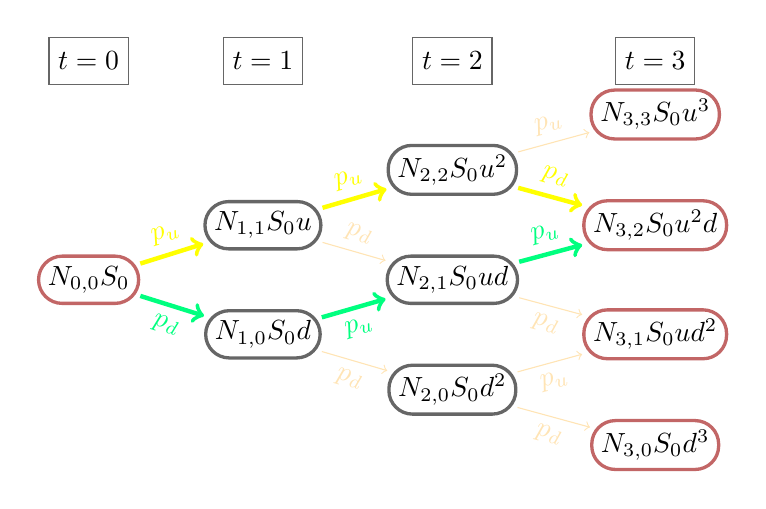
\begin{tikzpicture}
		\matrix[column sep=8mm,row sep=0.4mm,ampersand replacement=\&] (tree){
			\node[header] (t0) {$ t = 0 $};  \&  \node[header] (t1) {$ t = 1 $};  \&  \node[header] (t2) {$ t = 2 $};  \&  \node[header] (t3) {$ t = 3 $};  \\
			\&  \&  \& \node[term] (u3) {$ N_{3,3} \blacktriangleright S_0 u^3 $};  \\
			\&  \&  \node[nterm] (u2) {$ N_{2,2} \blacktriangleright S_0 u^2 $};  \&  \\
			\&  \node[nterm] (u) {$ N_{1,1} \blacktriangleright S_0 u $};  \&  \&  \node[term] (u2d) {$ N_{3,2} \blacktriangleright S_0 u^2 d $};  \\
			\node[term] (s) {$ N_{0,0} \blacktriangleright S_0 $};  \&  \&  \node[nterm] (ud) {$ N_{2,1} \blacktriangleright S_0 u d $};  \&  \\
			\&  \node[nterm] (d) {$ N_{1,0} \blacktriangleright S_0 d $};  \&  \&	\node[term] (ud2) {$ N_{3,1} \blacktriangleright S_0 u d^2 $};  \\
			\&  \&  \node[nterm] (d2) {$ N_{2,0} \blacktriangleright S_0 d^2 $};  \&  \\
			\&  \&  \& \node[term] (d3) {$ N_{3,0} \blacktriangleright S_0 d^3 $};  \\
		};
		
		% Lines out of s
		\draw[->,Yellow,ultra thick] (s) -- (u) node[midway,above,sloped] {$p_u$};
		\draw[->,SpringGreen,ultra thick] (s) -- (d) node[midway,below,sloped] {$p_d$};
		% Lines out of u
		\draw[->,Yellow,ultra thick] (u) -- (u2) node[midway,above,sloped] {$p_u$};
		\draw[->,Moccasin] (u) -- (ud) node[midway,above,sloped] {$p_d$};
		% Lines out of d
		\draw[->,SpringGreen,ultra thick] (d) -- (ud) node[midway,below,sloped] {$p_u$};
		\draw[->,Moccasin] (d) -- (d2) node[midway,below,sloped] {$p_d$};
		% Lines out of u2
		\draw[->,Moccasin] (u2) -- (u3) node[midway,above,sloped] {$p_u$};
		\draw[->,Yellow,ultra thick] (u2) -- (u2d) node[midway,above,sloped] {$p_d$};
		% Lines out of ud
		\draw[->,SpringGreen,ultra thick] (ud) -- (u2d) node[midway,above,sloped] {$p_u$};
		\draw[->,Moccasin] (ud) -- (ud2) node[midway,below,sloped] {$p_d$};
		% Lines out of d2
		\draw[->,Moccasin] (d2) -- (ud2) node[midway,below,sloped] {$p_u$};
		\draw[->,Moccasin] (d2) -- (d3) node[midway,below,sloped] {$p_d$};
		\end{tikzpicture}
		
		%		\caption{A 3-step recombinant tree}
		%		\label{fig:paths}
	\end{figure}
\end{frame}


\begin{frame}{\cite{Black1973} model (continuous)}
	\begin{description}
		\item[riskless] $ S_t^0 = e^{rt} $
		\item[risky] $ S_t  =  s_0 e^{ ( r - \frac{\sigma^2}{2} ) t + \sigma W_t } $
	\end{description}
	
	\begin{theorem}[Convergence of prices from CRR to BS]
		Prices of basic assets under CRR $ \xrightarrow{d} $ prices of basic assets under BS.
	\end{theorem}
	
	\begin{corollary}[Convergence of evaluation formulae]
		The previous theorem implies that evaluation formulae under CRR converge in distribution to evaluation formulae for BS.
	\end{corollary}
	
	\bigskip
	
	Approximate BS price by using CRR model.
	
	\bigskip
	
	\alert{Quest}: Find algorithms with reduced computational complexity.
	
\end{frame}


\begin{frame}{Market models: discrete vs. continuous}
	\begin{tabular}{lll}
		\toprule
		Parameter  &  Discrete  &  Continuous  \\
		\midrule
		Example  &  \cite{Cox1979}  &  \cite{Black1973}  \\
		Theoretical complexity  &  Easy  &  Hard  \\
		Ease of implementation  &  Hard  &  Easy  \\
		Closed-form formula  &  No\footnotemark  &  Yes  \\
		Computational complexity  &  Hard: $ O(2^n) $\footnotemark[1]  &  Easy: $ O(1) $  \\
		Universality  &  Yes  &  No  \\
		\bottomrule
	\end{tabular}
	\footnotetext{CRR: backward recursive}
\end{frame}



\section{Asian options}

\begin{frame}{Asian options}
	Payoff: function of some form of average price.
	
	\bigskip
	
	\begin{tabular}{lll}
		\toprule
		Average  &  Discrete  &  Continuous  \\
		\midrule
		AM  &  $ A_n = \frac{1}{n+1} \sum_{i=0}^{n} S_n $  &  $ A_T = \frac{1}{T} \int_{0}^{T} S_t \dif t $  \\
		GM  &  $ G_n = \left( \prod_{i=0}^{n} S_n \right)^{\frac{1}{n+1}} $  &  $  
		G_T = \exp \left(  \frac{1}{T} \int_{0}^{T} \log(S_t) \dif t  \right) $  \\
		\bottomrule
	\end{tabular}
	
	\bigskip
	
	\begin{example}[fixed-strike Asian call of European type]
		Given strike-price $ K $, payoff $ = (A_T - K)_+ $, exercised only at maturity.
	\end{example}	
\end{frame}


\begin{frame}{Asian option}{Pre-existing methods}
	\begin{block}{Arithmetic mean}
		\begin{tabular}{cccl}
			\toprule
			Method  &  Type  &  Complex  &  Remarks  \\
			\midrule
			\cite{Cox1979}  &  Tree  &  \alert{$ O(2^n) $}  &  simple, accurate, convergence  \\
			\cite{Hull1993}  &  Tree  &  $ O(n^3) $  &  accuracy \& convergence problems  \\
			\cite{Barraquand1996}  &  Tree  &  $ O(n^3) $  &  accuracy \& convergence problems  \\
			\cite{Chalasani1999}  &  Tree  &  $ O(n^4) $  &  thin bounds, very large memory  \\
			\cite{Vecer2001}  &  PDE  &  $ O(n^2) $  &  not universally applicable  \\
			\cite{dHalluin2005}  &  PDE  &    &  more general than \cite{Vecer2001} \\
			\bottomrule
		\end{tabular}
	\end{block}
	
	\bigskip
	
	\begin{block}{Geometric mean}
		Closed-form formula exist under BS.
	\end{block}
\end{frame}


\begin{frame}{SPs method for Asian options: Introduction}
	Idea: At any node $ N_{i,j} $:
	\begin{itemize}
		\item payoff $ P $: continuous, convex function of the underlying's average $ A $
		\item number of possible averages = number of paths to $ N_{i,j} $ = $ \binom{i}{j} $
		\item these averages completely characterise the payoff; no other payoff being possible under the given tree
		\item the above points $ ((A_{i,j}^l, P_{i,j}^l))_l $ are called \alert{singular points}
		\item payoff is represented as continuous, convex, and piecewise-linear function of the underlying's possible averages, found by joining the singular points
		\item minimum possible average $ A_{i,j}^{\min} = \frac{S_0}{i+1} \left( \frac{1 - d^{i-j+1}}{1-d} + d^{i-j} u \frac{1 - u^{j}}{1-u} \right)$
		\item maximum possible average $ A_{i,j}^{\max} = \frac{S_0}{i+1} \left( \frac{1 - u^{j+1}}{1-u} + u^{j} d \frac{1 - d^{i-j-1}}{1-d} \right) $
	\end{itemize}
\end{frame}


\begin{frame}{Singular Points method (SPM) for Asian option: Idea}
	\begin{description}
		\item[$ N_{i,j} $] Node of the binomial tree
		\item[$ A_{i,j} $] Average upto $ N_{i,j} $, $ \binom{i}{j} $ choices
		\item[$ P_{i,j} $] Option price at $ N_{i,j} $
		\item[$ \left\lbrace \left( A_{i,j}^l, P_{i,j}^l \right) \right\rbrace_l $] \alert{singular points} (SPs) -- completely characterise price
		\item[price] continuous, convex, piecewise-linear function found by joining SPs
	\end{description}
\end{frame}


\begin{frame}{SPM for Asian}{Start: at maturity ($ i = n $)}
	\begin{minipage}[t]{0.55\linewidth}
		At any node $ N_{n,j}, \exists $ three possibilities:
		\begin{enumerate}
			\item $ j \in \{ 0, n \} $: $ (A, (A-K)_+) $
			\item $ j \notin \{ 0, n \} $ and $ K \notin \left( A_{n,j}^{\min}, A_{n,j}^{\max} \right) $:
			\begin{enumerate}
				\item $ \left( A_{n,j}^{\min} , ( A_{n,j}^{\min} - K )_+ \right) $
				\item $ \left( A_{n,j}^{\max} , ( A_{n,j}^{\max} - K )_+ \right) $
			\end{enumerate}
			\item $ j \notin \{ 0, n \} $ and $ K \in \left( A_{n,j}^{\min}, A_{n,j}^{\max} \right) $: \begin{enumerate}
				\item $ ( A_{n,j}^{\min} , 0 ) $
				\item $ ( K , 0 ) $
				\item $ ( A_{n,j}^{\max} , A_{n,j}^{\max} - K ) $
			\end{enumerate}
		\end{enumerate}
	\end{minipage}
	\begin{minipage}[t]{0.40\linewidth}
		\begin{figure}
			\definecolor{zzffzz}{rgb}{0.6,1.,0.6}
			\definecolor{bfffqq}{rgb}{0.7490196078431373,1.,0.}
			\definecolor{ffffzz}{rgb}{1.,1.,0.6}
			\definecolor{ffffff}{rgb}{1.,1.,1.}
			\begin{tikzpicture}[line cap=round,line join=round,>=triangle 45,x=1.0cm,y=1.0cm]
			\draw[->,color=ffffff] (-0.5,0.) -- (3.5,0.);
			\foreach \x in {,1.,2.,3.}
			\draw[shift={(\x,0)},color=ffffff] (0pt,2pt) -- (0pt,-2pt);
			\draw[color=ffffff] (3.2339019240538707,0.05820970293171456) node [anchor=south west] { A};
			\draw[->,color=ffffff] (0.,-0.5) -- (0.,2.5);
			\foreach \y in {,1.,2.}
			\draw[shift={(0,\y)},color=ffffff] (2pt,0pt) -- (-2pt,0pt);
			\draw[color=ffffff] (0.0727621286646436,2.255161943734117) node [anchor=west] { P};
			\clip(-0.5,-0.5) rectangle (3.5,2.5);
			\draw [line width=2.pt,color=bfffqq] (1.5167156875682812,0.)-- (3.,1.5);
			\draw [line width=0.4pt,dash pattern=on 2pt off 2pt,color=ffffzz] (3.,1.5)-- (3.,0.);
			\draw [line width=2.pt,color=bfffqq] (0.49804588626327045,0.)-- (1.5167156875682812,0.);
			\draw [line width=0.4pt,dash pattern=on 2pt off 2pt,color=ffffzz] (3.,1.5)-- (0.,1.4984358056218274);
			\begin{scriptsize}
			\draw [fill=ffffzz] (1.5167156875682812,0.) circle (2.5pt);
			\draw[color=ffffzz] (1.5167156875682817,-0.3642746881930386) node {$K$};
			\draw [fill=ffffzz] (3.,1.5) circle (2.5pt);
			\draw [fill=ffffzz] (3.,0.) circle (1.5pt);
			\draw[color=ffffzz] (3.0156155380599396,-0.3060649852613241) node {$A_{i,j}^{\max}$};
			\draw [fill=ffffzz] (0.49804588626327045,0.) circle (2.5pt);
			\draw[color=ffffzz] (0.6290177178596299,-0.32061741099425267) node {$A_{i,j}^{\min}$};
			\draw [fill=zzffzz] (0.,1.4984358056218274) circle (2.5pt);
			\draw[color=zzffzz] (0.8618565295864893,1.2510445681620406) node {$\left( A_{i,j}^{\max} - K \right)_+$};
			\end{scriptsize}
			\end{tikzpicture}
			
			\caption{Case 3}
		\end{figure}		
	\end{minipage}
\end{frame}


\begin{frame}{SPM for Asian options: exact price}
	\begin{minipage}[t]{0.6\linewidth}
		\begin{itemize}
			\item Up movement (for $ N_{i,j} $):
			\begin{enumerate}
				\item $ \forall A_{i+1,j}^l: B^l = \frac{ ( i+2) A_{i+1,j}^l - S_{i+1,j} }{ i+1 } $.
				\item If $ B^l \in \left[ A_{i,j}^{\min}, A_{i,j}^{\max} \right]  \implies B^l $ is SA.
				\item For each SA, $ B^l_u = \frac{(i+1) B^l + S_{i+1,j+1}}{i+2} $.
				\item $ v_{i,j}( B^l ) = \frac{1}{R} \left[ p_u v_{i+1,j+1} \left( B^l_u \right) + p_d v_{i+1,j} \left( A_{i+1,j}^l \right) \right] $.
				\item $ \left( B^l, v_{i,j}( B^l ) \right) $ is a SP.
			\end{enumerate}
			\item Down movement (for $ N_{i,j} $).
			\item Aggregate and sort by SAs.
			\item Repeat for all $ j $.
			\item Iterate backward till $ i = 0 $. $ P_{0,0}^1 $ is the exact binomial price.
		\end{itemize}

	\end{minipage}
	\begin{minipage}[t]{0.3\linewidth}
		\begin{figure}
			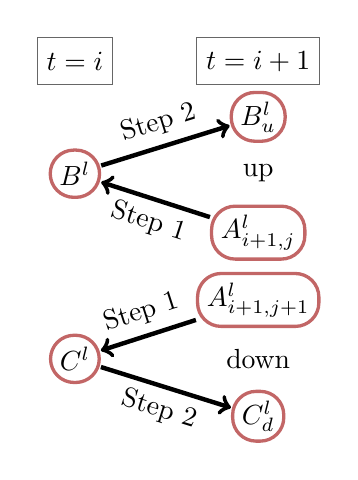
\begin{tikzpicture}
			\matrix (tree) [column sep=3em,row sep=0.2em,ampersand replacement=\&]{
				\node[header] (t0) {$ t = i $};  \&  \node[header] (t1) {$ t = i+1 $};  \\
				\&  \node[term] (u-u) {$ B^l_u $};  \\
				\node[term] (u-s) {$ B^l $};  \&  \node {up};  \\
				\&  \node[term] (u-d) {$ A_{i+1,j}^l $};  \\
				\\
				\&  \node[term] (d-u) {$ A_{i+1,j+1}^l $};  \\
				\node[term] (d-s) {$ C^l $};  \&  \node {down};  \\
				\&  \node[term] (d-d) {$ C^l_d $}; \\
			};
			\draw[->,ultra thick] (u-s) -- (u-u) node[midway,above,sloped] {Step 2};
			\draw[->,ultra thick] (u-d) -- (u-s) node[midway,below,sloped] {Step 1};
			\draw[->,ultra thick] (d-u) -- (d-s) node[midway,above,sloped] {Step 1};
			\draw[->,ultra thick] (d-s) -- (d-d) node[midway,below,sloped] {Step 2};
			\end{tikzpicture}
		\end{figure}
	\end{minipage}
\end{frame}


\begin{frame}{SPM for Asian options: American case}
	\definecolor{wqwqwq}{rgb}{0.3764705882352941,0.3764705882352941,0.3764705882352941}
	\definecolor{afeeee}{rgb}{0.6862745098039216,0.9333333333333333,0.9333333333333333}
	\definecolor{bcduew}{rgb}{0.7372549019607844,0.8313725490196079,0.9019607843137255}
	\definecolor{uququq}{rgb}{0.25098039215686274,0.25098039215686274,0.25098039215686274}
	\definecolor{dqfqcq}{rgb}{0.8156862745098039,0.9411764705882353,0.7529411764705882}
	\definecolor{ffffff}{rgb}{1.,1.,1.}
	\begin{tikzpicture}[line cap=round,line join=round,>=triangle 45,x=0.6cm,y=0.45cm]
	\draw[->,color=ffffff] (0.,0.) -- (17.,0.);
	\foreach \x in {,2.,4.,6.,8.,10.,12.,14.,16.}
	\draw[shift={(\x,0)},color=ffffff] (0pt,2pt) -- (0pt,-2pt);
	\draw[color=ffffff] (16.357213332379875,0.10062658140528619) node [anchor=south west] { A};
	\draw[->,color=ffffff] (0.,0.) -- (0.,15.);
	\foreach \y in {,2.,4.,6.,8.,10.,12.,14.}
	\draw[shift={(0,\y)},color=ffffff] (2pt,0pt) -- (-2pt,0pt);
	\draw[color=ffffff] (0.1257831816403861,14.001179347367474) node [anchor=west] { P};
	\clip(-1.,-1.) rectangle (17.,15.);
	\draw [line width=2.pt,color=dqfqcq] (6.,4.)-- (12.,8.);
	\draw [line width=2.pt,color=dqfqcq] (16.,12.)-- (12.,8.);
	\draw [line width=2.pt,color=dqfqcq] (6.,4.)-- (4.,3.);
	\draw [line width=2.pt,color=dqfqcq] (4.,3.)-- (1.,2.);
	\draw [line width=0.4pt,color=uququq] (12.,8.)-- (12.,0.);
	\draw [line width=0.4pt,color=uququq] (6.,4.)-- (6.,0.);
	\draw [line width=0.4pt,color=uququq] (4.,3.)-- (4.,0.);
	\draw [line width=0.4pt,color=uququq] (1.,2.)-- (1.,0.);
	\draw [line width=0.4pt,color=uququq] (16.,12.)-- (16.,0.);
	\draw [line width=2.pt,dash pattern=on 1pt off 1pt on 3pt off 4pt,color=afeeee] (8.003076923076923,5.335384615384616)-- (16.,13.33);
	\draw [line width=1.2pt,dash pattern=on 1pt off 1pt on 3pt off 4pt,color=afeeee] (2.66,0.)-- (8.003076923076923,5.335384615384616);
	\draw [color=wqwqwq] (8.003076923076923,5.335384615384616)-- (8.,0.);
	\draw [color=wqwqwq] (8.003076923076923,5.335384615384616)-- (0.,5.34);
	\begin{scriptsize}
	\draw [fill=dqfqcq] (16.,12.) circle (2.5pt);
	\draw[color=dqfqcq] (16.105646969099105,11.384888230830033) node {$S_5$};
	\draw [fill=dqfqcq] (12.,8.) circle (2.5pt);
	\draw[color=dqfqcq] (12.156055065590982,7.384981619969907) node {$S_4$};
	\draw [fill=dqfqcq] (6.,4.) circle (2.5pt);
	\draw[color=dqfqcq] (5.917209256227832,4.81900379413511) node {$S_3$};
	\draw [fill=dqfqcq] (4.,3.) circle (2.5pt);
	\draw[color=dqfqcq] (3.879521713653576,3.812737980082248) node {$S_2$};
	\draw[color=dqfqcq] (9.866801159735955,6.026522770998544) node {$f$};
	\draw [fill=dqfqcq] (1.,2.) circle (2.5pt);
	\draw[color=dqfqcq] (0.9865085359246955,2.756158875326743) node {$S_1$};
	\draw [fill=dqfqcq] (16.,0.) circle (1.5pt);
	\draw[color=dqfqcq] (16.005020423786796,-0.665144892452987) node {$A_5$};
	\draw [fill=dqfqcq] (12.,0.) circle (1.5pt);
	\draw[color=dqfqcq] (12.030271883950595,-0.665144892452987) node {$A_4$};
	\draw [fill=dqfqcq] (6.,0.) circle (1.5pt);
	\draw[color=dqfqcq] (6.093305710524372,-0.6148316017503439) node {$A_3$};
	\draw [fill=dqfqcq] (4.,0.) circle (1.5pt);
	\draw[color=dqfqcq] (4.005304895293962,-0.6148316017503439) node {$A_2$};
	\draw [fill=dqfqcq] (1.,0.) circle (1.5pt);
	\draw[color=dqfqcq] (0.9865085359246955,-0.5896749563990225) node {$A_1$};
	\draw [fill=bcduew] (8.003076923076923,5.335384615384616) circle (2.5pt);
	\draw[color=bcduew] (7.678173799193236,5.951052834944579) node {$\bar{S}$};
	\draw [fill=bcduew] (16.,13.33) circle (2.5pt);
	\draw[color=bcduew] (16.306900059723723,13.850239475259546) node {$S_5'$};
	\draw[color=afeeee] (11.829018793325979,10.1773692539666) node {$\bar{f}$};
	\draw [fill=afeeee] (2.66,0.) circle (1.5pt);
	\draw[color=afeeee] (2.6468465335777918,-0.6903015378043086) node {$K$};
	\draw [fill=afeeee] (8.,0.) circle (1.5pt);
	\draw[color=afeeee] (8.130993253098627,-0.6148316017503439) node {$\bar{A}$};
	\draw [fill=afeeee] (0.,5.34) circle (1.5pt);
	\draw[color=afeeee] (-0.17069673516685677,5.045413602297003) node {$\bar{P}$};
	\end{scriptsize}
	\end{tikzpicture}
\end{frame}


\begin{frame}{SPM for Asian options: Approximation}{Upper estimates}
	\definecolor{ffffqq}{rgb}{1.,1.,0.}
	\definecolor{dqfqcq}{rgb}{0.8156862745098039,0.9411764705882353,0.7529411764705882}
	\definecolor{wqwqwq}{rgb}{0.3764705882352941,0.3764705882352941,0.3764705882352941}
	\definecolor{afeeee}{rgb}{0.6862745098039216,0.9333333333333333,0.9333333333333333}
	\definecolor{ffffff}{rgb}{1.,1.,1.}
	\begin{tikzpicture}[line cap=round,line join=round,>=triangle 45,x=0.59cm,y=0.45cm]
	\draw[->,color=ffffff] (0.,0.) -- (17.,0.);
	\foreach \x in {,2.,4.,6.,8.,10.,12.,14.,16.}
	\draw[shift={(\x,0)},color=ffffff] (0pt,2pt) -- (0pt,-2pt);
	\draw[color=ffffff] (16.503014413215865,0.12712930521358398) node [anchor=south west] { A};
	\draw[->,color=ffffff] (0.,0.) -- (0.,13.);
	\foreach \y in {,2.,4.,6.,8.,10.,12.}
	\draw[shift={(0,\y)},color=ffffff] (2pt,0pt) -- (-2pt,0pt);
	\draw[color=ffffff] (0.158911605284918,12.306834374720044) node [anchor=west] { P};
	\clip(-1.,-1.) rectangle (17.,13.);
	\draw [line width=2.pt,color=afeeee] (16.,12.)-- (12.05,7.25);
	\draw [line width=2.pt,color=afeeee] (8.053489465238158,3.603050081817436)-- (4.,2.5);
	\draw [line width=2.pt,color=afeeee] (4.,2.5)-- (1.,2.);
	\draw [line width=0.4pt,color=wqwqwq] (12.05,7.25)-- (12.,0.);
	\draw [line width=0.4pt,color=wqwqwq] (8.053489465238158,3.603050081817436)-- (8.,0.);
	\draw [line width=0.4pt,color=wqwqwq] (4.,2.5)-- (4.,0.);
	\draw [line width=0.4pt,color=wqwqwq] (1.,2.)-- (1.,0.);
	\draw [line width=2.pt,dash pattern=on 1pt off 1pt on 2pt off 4pt,color=dqfqcq] (4.,2.5)-- (12.05,7.25);
	\draw [line width=0.4pt,color=wqwqwq] (16.,12.)-- (16.,0.);
	\draw [line width=1.2pt,dotted,color=ffffqq] (8.025,4.875)-- (8.053489465238158,3.603050081817436);
	\draw [line width=2.pt,color=afeeee] (8.053489465238158,3.603050081817436)-- (12.05,7.25);
	\draw [color=dqfqcq](2.487010827086094,9.891377575661947) node[anchor=north west] {$f_u(A) \ge f(A) \quad \forall A$};
	\draw [color=ffffqq](2.518793148143078,8.397608239402336) node[anchor=north west] {$(f_u - f)(A) \le \varepsilon \quad \forall A$};
	\begin{scriptsize}
	\draw [fill=afeeee] (16.,12.) circle (2.0pt);
	\draw[color=afeeee] (16.40766745004491,11.512276217135144) node {$S_5$};
	\draw [fill=afeeee] (12.05,7.25) circle (2.0pt);
	\draw[color=afeeee] (12.434877317921963,6.840274250535932) node {$S_4$};
	\draw [fill=afeeee] (8.053489465238158,3.603050081817436) circle (2.0pt);
	\draw[color=afeeee] (8.430304864742027,3.1217420730386003) node {$S_3$};
	\draw [fill=afeeee] (4.,2.5) circle (2.0pt);
	\draw[color=afeeee] (4.362167769448127,2.041142978723137) node {$S_2$};
	\draw[color=afeeee] (6.396236317095077,2.8039188100046406) node {f};
	\draw [fill=afeeee] (1.,2.) circle (2.0pt);
	\draw[color=afeeee] (1.4064119111486517,1.6915373893857808) node {$S_1$};
	\draw [fill=afeeee] (16.,0.) circle (2.0pt);
	\draw[color=afeeee] (16.185191202646024,-0.43787847294175086) node {$A_5$};
	\draw [fill=afeeee] (12.,0.) circle (2.0pt);
	\draw[color=afeeee] (12.117054107352125,-0.4696607992451468) node {$A_4$};
	\draw [fill=afeeee] (8.,0.) circle (2.0pt);
	\draw[color=afeeee] (8.080699333115207,-0.5332254518519388) node {$A_3$};
	\draw [fill=afeeee] (4.,0.) circle (2.0pt);
	\draw[color=afeeee] (4.04434455887829,-0.5650077781553349) node {$A_2$};
	\draw [fill=afeeee] (1.,0.) circle (2.0pt);
	\draw[color=afeeee] (1.056806379521832,-0.5332254518519388) node {$A_1$};
	\draw[color=dqfqcq] (9.002386643767732,6.109280745557824) node {$f_u$};
	\draw [fill=dqfqcq] (8.025,4.875) circle (2.0pt);
	\draw[color=dqfqcq] (7.508617554089503,5.092246303849152) node {$R_3$};
	\draw[color=ffffqq] (8.398522543685043,4.265905819960856) node {$\varepsilon_3$};
	\draw[color=afeeee] (10.464373412388976,5.314722587972924) node {f};
	\end{scriptsize}
	\end{tikzpicture}
\end{frame}


\begin{frame}{SPM for Asian options: Approximation}{Lower estimates}
	\definecolor{ffffqq}{rgb}{1.,1.,0.}
	\definecolor{wqwqwq}{rgb}{0.3764705882352941,0.3764705882352941,0.3764705882352941}
	\definecolor{afeeee}{rgb}{0.6862745098039216,0.9333333333333333,0.9333333333333333}
	\definecolor{ffffff}{rgb}{1.,1.,1.}
	\begin{tikzpicture}[line cap=round,line join=round,>=triangle 45,x=0.59cm,y=0.45cm]
	\draw[->,color=ffffff] (0.,0.) -- (17.,0.);
	\foreach \x in {,2.,4.,6.,8.,10.,12.,14.,16.}
	\draw[shift={(\x,0)},color=ffffff] (0pt,2pt) -- (0pt,-2pt);
	\draw[color=ffffff] (16.983734759565976,0.15704689406799202) node [anchor=south west] { A};
	\draw[->,color=ffffff] (0.,0.) -- (0.,13.);
	\foreach \y in {,2.,4.,6.,8.,10.,12.}
	\draw[shift={(0,\y)},color=ffffff] (2pt,0pt) -- (-2pt,0pt);
	\draw[color=ffffff] (0.19630858508193877,12.246817877668772) node [anchor=west] { P};
	\clip(-1.,-1.) rectangle (17.,13.);
	\draw [line width=2.pt,color=afeeee] (4.,2.5)-- (12.,8.);
	\draw [line width=2.pt,color=afeeee] (16.,12.)-- (12.,8.);
	\draw [line width=0.4pt,color=wqwqwq] (12.,8.)-- (12.,0.);
	\draw [line width=0.4pt,color=wqwqwq] (4.,2.5)-- (4.,0.);
	\draw [line width=0.4pt,color=wqwqwq] (1.,2.)-- (1.,0.);
	\draw [line width=2.pt,dash pattern=on 2pt off 2pt,color=afeeee] (4.,2.5)-- (7.,3.);
	\draw [line width=2.pt,dash pattern=on 2pt off 2pt,color=afeeee] (12.,8.)-- (7.,3.);
	\draw [line width=0.4pt,color=wqwqwq] (7.,3.)-- (6.998942733420039,0.);
	\draw [line width=0.4pt,color=wqwqwq] (16.,12.)-- (16.,0.);
	\draw [line width=1.2pt,dash pattern=on 1pt off 1pt,color=ffffqq] (7.000519372007349,4.562857068255052)-- (7.,3.);
	\draw [color=afeeee](1.9857588593058553,11.540106854362808) node[anchor=north west] {$f_d(A) \le f(A) \quad \forall A$};
	\draw [color=ffffqq](1.9857588593058553,10.48004031940386) node[anchor=north west] {$(f - f_d) (A) \le \delta  \quad  \forall A$};
	\draw [line width=2.pt,color=afeeee] (1.,2.)-- (4.,2.5);
	\begin{scriptsize}
	\draw [fill=afeeee] (16.,12.) circle (2.0pt);
	\draw[color=afeeee] (16.355547287303775,11.500845130845809) node {$S_4$};
	\draw [fill=afeeee] (12.,8.) circle (2.0pt);
	\draw[color=afeeee] (12.429375585664998,7.260578991010025) node {$S_3$};
	\draw [fill=afeeee] (4.,2.5) circle (2.0pt);
	\draw[color=afeeee] (4.4592470313382835,2.03876976324929) node {$S_2$};
	\draw [fill=afeeee] (1.,2.) circle (2.0pt);
	\draw[color=afeeee] (1.2790479530108758,1.5283673575283159) node {$S_1$};
	\draw [fill=afeeee] (16.,0.) circle (2.0pt);
	\draw[color=afeeee] (16.041453551172673,-0.7095508829405706) node {$A_4$};
	\draw [fill=afeeee] (12.,0.) circle (2.0pt);
	\draw[color=afeeee] (12.076020132517508,-0.6702891594235725) node {$A_3$};
	\draw [fill=afeeee] (4.,0.) circle (2.0pt);
	\draw[color=afeeee] (4.105891578190794,-0.6702891594235725) node {$A_2$};
	\draw [fill=afeeee] (1.,0.) circle (2.0pt);
	\draw[color=afeeee] (1.0042159338961614,-0.7488126064575684) node {$A_1$};
	\draw [fill=afeeee] (6.998942733420039,0.) circle (2.0pt);
	\draw[color=afeeee] (7.011258637403488,-0.7095508829405706) node {$A_{23}$};
	\draw [fill=afeeee] (7.,3.) circle (2.0pt);
	\draw[color=afeeee] (7.482399241600141,2.156554933800284) node {$R_{23}$};
	\draw[color=afeeee] (5.833407126911855,2.156554933800284) node {$f_d$};
	\draw[color=afeeee] (9.798840545567018,4.9441373035071425) node {$f_d$};
	\draw [fill=afeeee] (7.000519372007349,4.562857068255052) circle (2.0pt);
	\draw[color=afeeee] (6.5793797502232225,5.925680391432093) node {$S_{23}$};
	\draw[color=ffffqq] (7.286090656518202,3.7270238744802042) node {$\delta_4$};
	\end{scriptsize}
	\end{tikzpicture}
\end{frame}


\begin{frame}{Singular points method for Asian options}{Numerical results}
	Data: $ s_0 = 100, T = 1, r = 0.1, q = 0.03 $.
	\begin{tabular}{crcccc}
		\toprule
		&         &  \multicolumn{2}{c}{$ K = 90 $}  &  \multicolumn{2}{c}{$ K = 110 $}  \\
		\cmidrule(lr){3-4}\cmidrule(lr){5-6}
		&  $ n $  &  $ \sigma = 0.2 $  &  $ \sigma = 0.4 $  &  $ \sigma = 0.2 $  &  $ \sigma = 0.4 $  \\
		\midrule
		\multirow{2}{2em}{Bin}
		&   10  &  14.5912  &  17.8033  &  2.5100  &  6.6523  \\
		&   25  &  15.1535  &  18.6786  &  2.6270  &  7.3451  \\
		\midrule
		\multirow{6}{2em}{SP}
		&   10  &  14.5925  &  17.8068  &  2.5090  &  6.6511  \\
		&   25  &  15.1535  &  18.6785  &  2.6270  &  7.3449  \\
		&   50  &  15.3524  &  19.0420  &  2.6673  &  7.4563  \\
		&  100  &  15.4732  &  19.2696  &  2.6886  &  7.5174  \\
		&  200  &  15.5453  &  19.4065  &  2.6996  &  7.5502  \\
		&  400  &  15.5861  &  19.4845  &  2.7053  &  7.5674  \\
		\bottomrule
	\end{tabular}
\end{frame}


\begin{frame}{SPM for Asian options: summary}
	\begin{itemize}
		\neu Introduced by Gaudenzi \emph{et al} \cite{Gaudenzi2010} in 2010.
		\pro Convergent to exact CRR and thus BS.
		\pro Easily generalised to American case and lookback options.
		\pro Approx: unnecessary points $ \implies $ selective removal.
		\pro Approx: \emph{A priori} error bounds.
		\pro Approx $ \implies $ fast: reduction of complexity from exponential time to polynomial time (experimental) of $ O(n^3) $.
		\con Difficult to compute theoretical complexity.
		\con Depends on the recombinant nature of the underlying's tree.
		\con<alert@1-> Not extensible to GM, since the price function is non-linear. $ G_u = \left( G^{i+1} S_{i+1,j} \right)^{\frac{1}{i+2}} \propto G^{\frac{i+1}{i+2}} $
		\con<alert@1-> Constant volatility assumption $ \implies $ local volatility models fail.
	\end{itemize}
\end{frame}



\section{Cliquet options}

\begin{frame}{Cliquet options: introduction}
	\begin{block}{Definitions}
		\begin{description}
			\item[forward start option] price option today with payoff $ = (S_T - S_u)_+ $, $ 0 \le u < T $.
			\item[cliquet option] a series of consecutive at-the-money forward start options, with bounded returns.
		\end{description}
	\end{block}
	\begin{block}{Pros and cons}
		\begin{itemize}
			\pro Safety against downside risks.
			\pro Significant upside potential.
			\con Unbounded gains not possible.
		\end{itemize}
	\end{block}
\end{frame}


\begin{frame}{Cliquet options: terminology \& literature review}
	\begin{block}{Terminology}
		\begin{itemize}
			\item Observation times: time points at which the forward start options expire. Assumption: equidistant.
			\item Return: $ R_i = \frac{S_i - S_{i-1}}{S_{i-1}} = \frac{S_i}{S_{i-1}} - 1 $.
			\item Running sum: $ Z_i = \sum_{k = 1}^{i} \max \{ F_{loc}, \min \{ C_{loc}, R_k \} \} $.
			\item $ \mathrm{Payoff} = \mathrm{notional} \cdot \max \{ F_{glob}, \min \{ C_{glob}, Z_{N} \} \} $.
		\end{itemize}
	\end{block}	
	\begin{block}{Pre-existing methods for pricing}
		\begin{itemize}
			\item No prominent tree-based method.
			\item \cite{Wilmott2002}: PDE based, FD approach.
			\item \cite{Windcliff2006}: PDE based, FD approach; generalisations.
		\end{itemize}
	\end{block}
\end{frame}


\begin{frame}{SPM for cliquet options: details}
	Idea: At the $ i $\textsuperscript{th} interval:
	\begin{itemize}
		\item $ m $: number of computational steps
		\item $ 2^m $ possible paths; probability -- binomially distributed.
		\item $ Z $ (running sum) depends on paths and their probabilities.
		\item $ (Z, P) \implies $ SP, where $ P \implies $ price function.
	\end{itemize}
	Price function at maturity: piecewise-linear, continuous (not convex).
	
	\begin{figure}
		\definecolor{wqwqwq}{rgb}{0.3764705882352941,0.3764705882352941,0.3764705882352941}
		\definecolor{afeeee}{rgb}{0.6862745098039216,0.9333333333333333,0.9333333333333333}
		\definecolor{dqfqcq}{rgb}{0.8156862745098039,0.9411764705882353,0.7529411764705882}
		\definecolor{ffffff}{rgb}{1.,1.,1.}
		\begin{tikzpicture}[line cap=round,line join=round,>=triangle 45,x=1.0cm,y=1.0cm]
		\draw[->,color=ffffff] (0.,0.) -- (6.,0.);
		\foreach \x in {,1.,2.,3.,4.,5.}
		\draw[shift={(\x,0)},color=ffffff] (0pt,2pt) -- (0pt,-2pt);
		\draw[color=ffffff] (5.780966613571441,0.054247335995569544) node [anchor=south west] { Z};
		\draw[->,color=ffffff] (0.,0.) -- (0.,3.5);
		\foreach \y in {,1.,2.,3.}
		\draw[shift={(0,\y)},color=ffffff] (2pt,0pt) -- (-2pt,0pt);
		\draw[color=ffffff] (0.06780919373316127,3.2068898782737656) node [anchor=west] { P};
		\clip(-1.,-0.5) rectangle (6.,3.5);
		\draw [line width=2.pt,color=dqfqcq] (1.,1.)-- (2.,1.);
		\draw [line width=2.pt,color=dqfqcq] (2.,1.)-- (4.,3.);
		\draw [line width=2.pt,color=dqfqcq] (4.,3.)-- (5.,3.);
		\draw [line width=0.4pt,color=wqwqwq] (1.,1.)-- (1.,0.);
		\draw [line width=0.4pt,color=wqwqwq] (2.,1.)-- (2.,0.);
		\draw [line width=0.4pt,color=wqwqwq] (4.,3.)-- (4.,0.);
		\draw [line width=0.4pt,color=wqwqwq] (5.,3.)-- (5.,0.);
		\draw [line width=0.4pt,color=wqwqwq] (1.,1.)-- (0.,1.);
		\draw [line width=0.4pt,color=wqwqwq] (4.,3.)-- (0.,3.);
		\begin{scriptsize}
		\draw [fill=dqfqcq] (1.,1.) circle (2.5pt);
		\draw[color=dqfqcq] (0.9258283422770939,1.4438514584177555) node {$S_1$};
		\draw [fill=dqfqcq] (2.,1.) circle (2.5pt);
		\draw[color=dqfqcq] (1.7666623445682936,1.4438514584177555) node {$S_2$};
		\draw [fill=dqfqcq] (4.,3.) circle (2.5pt);
		\draw[color=dqfqcq] (4.2077933189621,2.6237310163213934) node {$S_3$};
		\draw [fill=dqfqcq] (5.,3.) circle (2.5pt);
		\draw[color=dqfqcq] (5.170683869972989,2.6644165183180704) node {$S_4$};
		\draw [fill=afeeee] (1.,0.) circle (1.5pt);
		\draw[color=afeeee] (0.8580191485439326,-0.3191869614382546) node {$F_{loc} N_{obs}$};
		\draw [fill=afeeee] (2.,0.) circle (1.5pt);
		\draw[color=afeeee] (2.065022796994203,-0.3191869614382546) node {$F_{glob}$};
		\draw [fill=afeeee] (4.,0.) circle (1.5pt);
		\draw[color=afeeee] (3.963680221522719,-0.3191869614382546) node {$C_{glob}$};
		\draw [fill=afeeee] (5.,0.) circle (1.5pt);
		\draw[color=afeeee] (5.035065482506667,-0.3191869614382546) node {$C_{loc} N_{obs}$};
		\draw [fill=afeeee] (0.,1.) circle (1.5pt);
		\draw[color=afeeee] (-0.17268059620011877,0.8742544304642753) node {$F_{glob}$};
		\draw [fill=afeeee] (0.,3.) circle (1.5pt);
		\draw[color=afeeee] (-0.22692795118664777,2.908529530298133) node {$C_{glob}$};
		\end{scriptsize}
		\end{tikzpicture}
	\end{figure}
\end{frame}


\begin{frame}{SPM for cliquet options: other times ($ i < N $)}
	The realizable paths and associated quantities are denoted by primed variables.
	\begin{enumerate}
		\item From running sums $ Z_{i+1}^l $, subtract possible returns $ R_j' $ to get $ B_{l,j} $.
		\item If $ B_{l,j} \in [ i F_{loc}, i C_{loc} ] \implies $ singular point at time $ i $.
		\item Price function: $ v_i (B_{l,j}) = e^{- \frac{rT}{N}} \sum_{j=0}^{j_0} \left[ p_j' v_{i+1} (Z + R_j') \right] $.
		\item Linear combination of piecewise-linear continuous functions is piecewise-linear and continuous. Iterate backward.
		\item $ v_0 (B_{0,0}) $ is the exact binomial price.
	\end{enumerate}
\end{frame}


\begin{frame}{SPM for cliquet options: Approximation}
	\definecolor{ffffqq}{rgb}{1.,1.,0.}
	\definecolor{qqffqq}{rgb}{0.,1.,0.}
	\definecolor{wqwqwq}{rgb}{0.3764705882352941,0.3764705882352941,0.3764705882352941}
	\definecolor{eqeqeq}{rgb}{0.8784313725490196,0.8784313725490196,0.8784313725490196}
	\definecolor{dqfqcq}{rgb}{0.8156862745098039,0.9411764705882353,0.7529411764705882}
	\definecolor{afeeee}{rgb}{0.6862745098039216,0.9333333333333333,0.9333333333333333}
	\definecolor{ffffff}{rgb}{1.,1.,1.}
	\begin{tikzpicture}[line cap=round,line join=round,>=triangle 45,x=0.8cm,y=0.8cm]
	\draw[->,color=ffffff] (0.,0.) -- (12.,0.);
	\foreach \x in {,1.,2.,3.,4.,5.,6.,7.,8.,9.,10.,11.}
	\draw[shift={(\x,0)},color=ffffff] (0pt,2pt) -- (0pt,-2pt);
	\draw[color=ffffff] (11.72949600014192,0.0665249798016828) node [anchor=south west] { Z};
	\draw[->,color=ffffff] (0.,0.) -- (0.,8.);
	\foreach \y in {,1.,2.,3.,4.,5.,6.,7.}
	\draw[shift={(0,\y)},color=ffffff] (2pt,0pt) -- (-2pt,0pt);
	\draw[color=ffffff] (0.08315628750088702,7.641135707448683) node [anchor=west] { P};
	\clip(-1.,-1.) rectangle (12.,8.);
	\draw [line width=2.pt,color=dqfqcq] (1.,1.)-- (2.,1.);
	\draw [line width=1.6pt,dash pattern=on 1pt off 2pt on 3pt off 4pt,color=eqeqeq] (2.,1.)-- (3.,1.75);
	\draw [line width=1.6pt,dash pattern=on 1pt off 2pt on 3pt off 4pt,color=eqeqeq] (3.,1.75)-- (4.,2.);
	\draw [color=wqwqwq] (1.,1.)-- (1.,0.);
	\draw [color=wqwqwq] (2.,1.)-- (2.,0.);
	\draw [color=wqwqwq] (3.,1.75)-- (3.,0.);
	\draw [color=wqwqwq] (4.,2.)-- (4.,0.);
	\draw [color=wqwqwq] (1.,1.)-- (0.,1.);
	\draw [line width=1.6pt,dash pattern=on 1pt off 2pt on 3pt off 4pt,color=eqeqeq] (4.,2.)-- (6.,2.75);
	\draw [line width=1.6pt,dash pattern=on 1pt off 2pt on 3pt off 4pt,color=eqeqeq] (8.,4.)-- (9.,5.);
	\draw [line width=2.pt,color=dqfqcq] (9.,5.)-- (10.,7.);
	\draw [color=wqwqwq] (6.,2.75)-- (6.,0.);
	\draw [color=wqwqwq] (9.,5.)-- (9.,0.);
	\draw [color=wqwqwq] (11.,7.)-- (11.,0.);
	\draw [line width=1.6pt,dash pattern=on 1pt off 2pt on 3pt off 4pt,color=eqeqeq] (6.,2.75)-- (8.,4.);
	\draw [color=wqwqwq] (8.,4.)-- (8.,0.);
	\draw [color=wqwqwq] (10.,7.)-- (10.,0.);
	\draw [line width=2.pt,color=dqfqcq] (10.,7.)-- (11.,7.);
	\draw [line width=2.pt,color=dqfqcq] (2.,1.)-- (9.,5.);
	\draw [line width=1.6pt,dash pattern=on 3pt off 3pt,color=afeeee] (2.,1.)-- (10.,7.);
	\draw [line width=1.6pt,dotted,color=qqffqq] (6.004094596374262,3.288054055071007)-- (6.,2.75);
	\draw [color=wqwqwq] (10.,7.)-- (0.,7.);
	\draw [line width=1.6pt,dotted,color=ffffqq] (7.999695997451529,5.499771998088647)-- (8.,4.);
	\draw [color=qqffqq](1.0023349125274963,6.194217396762082) node[anchor=north west] {$| (V_1 - V)(Z) | \le h  \quad  \forall Z$};
	\draw [color=ffffqq](1.0023349125274963,5.19634269973684) node[anchor=north west] {$\exists Z \: | (V_2 - V)(Z) | > h$};
	\begin{scriptsize}
	\draw [fill=afeeee] (1.,1.) circle (2.0pt);
	\draw[color=afeeee] (0.9857036550273188,1.3877876060904992) node {$S_1$};
	\draw [fill=afeeee] (2.,1.) circle (2.0pt);
	\draw[color=afeeee] (1.8338977875363665,1.4376813409417613) node {$S_2$};
	\draw [fill=afeeee] (3.,1.75) circle (2.0pt);
	\draw[color=afeeee] (2.9149295250478975,2.0862998940081687) node {$S_3$};
	\draw [fill=afeeee] (4.,2.) circle (2.0pt);
	\draw[color=afeeee] (4.212167610061735,1.6705187702476512) node {$S_4$};
	\draw [fill=afeeee] (1.,0.) circle (2.0pt);
	\draw[color=afeeee] (0.9191786250266092,-0.35849311370367437) node {$Z_1$};
	\draw [fill=afeeee] (2.,0.) circle (2.0pt);
	\draw[color=afeeee] (1.9503165900376083,-0.3252306238028329) node {$Z_2$};
	\draw [fill=afeeee] (3.,0.) circle (2.0pt);
	\draw[color=afeeee] (2.9481920400482524,-0.3252306238028329) node {$Z_3$};
	\draw [fill=afeeee] (4.,0.) circle (2.0pt);
	\draw[color=afeeee] (3.929436232558719,-0.35849311370367437) node {$Z_4$};
	\draw [fill=afeeee] (0.,1.) circle (2.0pt);
	\draw[color=afeeee] (0.037721977517206906,0.7558002979745126) node {$F_{glob}$};
	\draw [fill=afeeee] (0.,7.) circle (2.0pt);
	\draw[color=afeeee] (0.004459462516852086,6.7264172351755445) node {$C_{glob}$};
	\draw [fill=afeeee] (6.,2.75) circle (2.0pt);
	\draw[color=afeeee] (6.174655995082668,2.302506078363638) node {$S_5$};
	\draw [fill=afeeee] (8.,4.) circle (2.0pt);
	\draw[color=afeeee] (8.15377563760378,3.5997431844964525) node {$S_6$};
	\draw [fill=afeeee] (9.,5.) circle (2.0pt);
	\draw[color=afeeee] (9.218176117615133,4.597617881521694) node {$S_7$};
	\draw [fill=afeeee] (10.,7.) circle (2.0pt);
	\draw[color=afeeee] (10.166157795125246,6.560104785671337) node {$S_8$};
	\draw [fill=afeeee] (11.,7.) circle (2.0pt);
	\draw[color=afeeee] (11.197295760136244,6.576736030621758) node {$S_9$};
	\draw [fill=afeeee] (6.,0.) circle (2.0pt);
	\draw[color=afeeee] (5.9584496475803626,-0.30859937885241223) node {$Z_5$};
	\draw [fill=afeeee] (8.,0.) circle (2.0pt);
	\draw[color=afeeee] (7.95420054760165,-0.3252306238028329) node {$Z_6$};
	\draw [fill=afeeee] (9.,0.) circle (2.0pt);
	\draw[color=afeeee] (8.952075997612294,-0.3418618687532536) node {$Z_7$};
	\draw [fill=afeeee] (11.,0.) circle (2.0pt);
	\draw[color=afeeee] (10.89793312513305,-0.3418618687532536) node {$Z_9$};
	\draw [fill=afeeee] (10.,0.) circle (2.0pt);
	\draw[color=afeeee] (9.933320190122762,-0.3252306238028329) node {$Z_8$};
	\draw[color=dqfqcq] (6.540543660086572,3.8658431037031837) node {$V_1$};
	\draw[color=afeeee] (5.559299467576104,3.9822618183561285) node {$V_2$};
	\draw [color=qqffqq] (6.004094596374262,3.288054055071007)-- ++(-2.0pt,-2.0pt) -- ++(4.0pt,4.0pt) ++(-4.0pt,0) -- ++(4.0pt,-4.0pt);
	\draw[color=qqffqq] (6.340968570084443,3.0841745910334106) node {$\le$ h};
	\draw [color=ffffqq] (7.999695997451529,5.499771998088647)-- ++(-1.5pt,-1.5pt) -- ++(3.0pt,3.0pt) ++(-3.0pt,0) -- ++(3.0pt,-3.0pt);
	\draw[color=ffffqq] (8.303456955105375,4.847086555778005) node {>h};
	\end{scriptsize}
	\end{tikzpicture}
\end{frame}


\begin{frame}{SPM for cliquet options: Numerical results}
	\begin{block}{Data}
		\begin{itemize}
			\item $ F_{loc} = 0, C_{loc} = 0.08, F_{glob} = 0.16, C_{glob} = \infty $
			\item $ T = 5, N = 5, r = 0.03 $
		\end{itemize}
	\end{block}
	
	\begin{tabular}{rrcccc}
		\toprule\multirow{2}{1em}{$ \sigma $}  &  \multirow{2}{1em}{$ m $}
		&  \multicolumn{2}{c}{Price}  &  \multicolumn{2}{c}{Time (s)}\footnote{$ \infty $ means time taken is more than an hour.}  \\
		\cmidrule(lr){3-4}\cmidrule(lr){5-6}
		&&  Bin  &  SP  &  Bin  &  SP  \\
		\midrule
		\multirow{3}{1em}{$ 0.2 $}
		&   200  &  0.173716366  &  0.173716366  &  0.0165  &  0.00828  \\
		&   500  &  0.173922597  &  0.173922671  &  0.0875  &  0.0437  \\
		&  1000  &  0.174051949  &  0.174051983  &  2.38  &  0.183  \\
		\midrule
		\multirow{3}{1em}{$ 0.02 $}
		&   200  &  0.150465004  &  0.150466828  &  600  &  6.09  \\
		&   500  &  0.150508871  &  0.150510526  &  $ \infty $  &  24.2  \\
		&  1000  &  0.150522368  &  0.150524027  &  $ \infty $  &  55  \\
		\bottomrule
	\end{tabular}	
\end{frame}


\begin{frame}{SPM for cliquet options: complexity -- $ O(m^2) $}
	% This plot was generated by plotly
	\begin{figure}
		\centering
		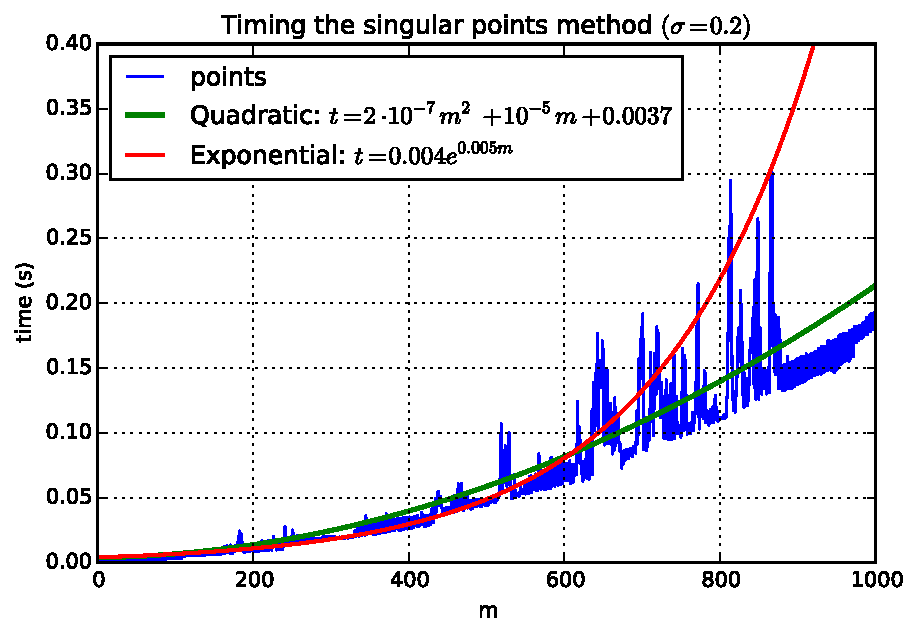
\includegraphics[height=0.75\textheight,width=\textwidth]{../img/timing-cliquet}
	\end{figure}
\end{frame}


\begin{frame}{SPM for cliquet options: Summary}
	\begin{itemize}
		\neu Introduced by Gaudenzi \emph{et al} \cite{Gaudenzi2011} in 2011.
		\pro Convergent to exact CRR and thus BS.
		\pro Approximation -- \emph{A priori} error bounds.
		\pro Significant speed improvement in low volatility cases against binomial model.
		\pro<alert@1-> Can be used for local volatility models and varying interest rates in each period.
		\pro<alert@1-> Fast -- experimental order of complexity $ O(m^2) $.
		\con Difficult to compute theoretical complexity.
	\end{itemize}
\end{frame}


\section{Conclusion}

\begin{frame}{Recapitulation}
	\begin{itemize}
		\item Efficient technique to evaluate path-dependent exotic options.
		\item Theory varies with option type.
		\item Asian: the method is complicated and is not flexible, although being fast and efficient. Easily generalised to the American case and to lookback options. \alert{Fails to be generalised for geometric mean and local volatility models.}
		\item Cliquet: flexible method; takes care of local volatility and interest rates. \alert{We found out that computational complexity (experimental) is approximately $ O(m^2) $ for low $ m $}.
	\end{itemize}
	
	Further research
	\begin{itemize}
		\item Theoretical complexity: dependence of singular point redundancy on initial data.
		\item Customising the method for other path-dependent options.
	\end{itemize}
\end{frame}


\begin{frame}[plain,c]
	
	\begin{center}
		{\Huge Questions?}
	\end{center}
	
	\vfill
	
	\begin{center}
		{\Huge Thank you!}
	\end{center}
	
\end{frame}


\appendix
%\section<presentation>*{\appendixname}
%\subsection<presentation>*{Bibliography}

\begin{frame}[allowframebreaks]
	\frametitle<presentation>{Bibliography}
	\printbibliography
\end{frame}


\end{document}
